\section{Background}
\subsection{CERN}
CERN (European Organisation for Nuclear Research) \cite{CERN_official} is the world's largest particle physics laboratory. Founded in 1954, it is located at the Swiss-French border near Geneva. Today, more than 100 countries participate in CERN and more than 11 thousand people affiliated with CERN.

The guiding ambition behind CERN is to deepen humanity's understanding of the universe by studying the components of matter and the forces holding them together. Numerous experiments target a large variety of problems, ranging from nuclear to high-energy physics, from studies of antimatter and cancer treatment to the possible effects of cosmic rays on clouds.

It is noteworthy that in 2012 CERN announced the observation of a new particle, the Higgs boson, as proposed within the Standard Model \cite{CERN_higgs}, leading to a Nobel prize for Dr. Peter Higgs (University of Edinburgh) and Dr. François Englert (University of Brussels). 

\subsection{The LHC}
The LHC (Large Hadron Collider), at CERN, consists of a 27-kilometre ring of superconducting magnets, 100 metres below the earth's surface (figure \ref{fig:LHC}). Inside of it, a number of accelerating structures boost the energy of two high-energy particle beams that travel opposite to each other, at close to the speed of light, before they are made to collide.  

\begin{figure}
    \centering
    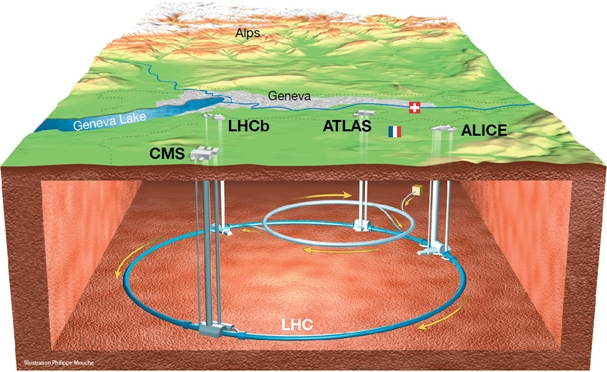
\includegraphics[width=0.9\linewidth]{images/LHC.jpg}
        \caption{A visual representation of the LHC at CERN. Above ground the four biggest particle detectors can be seen. Taken from \cite{CERN_official}.}
    \label{fig:LHC}
\end{figure}

There are four collision locations along the LHC, corresponding to the positions of four massive particle detectors, and therefore four experiments. Tens of millions of collisions take place every second at those locations, creating a dense particle plasma, the same that is speculated to have been present just seconds after the Big Bang occurred.

\subsection{ATLAS}
The ATLAS (A Toroidal LHC ApparatuS) experiment\cite{aad2008atlas} at CERN  investigates a wide range of physics, from the search for the Higgs boson to extra dimensions and particles that could make up dark matter.

\begin{figure}[t]
    \centering
    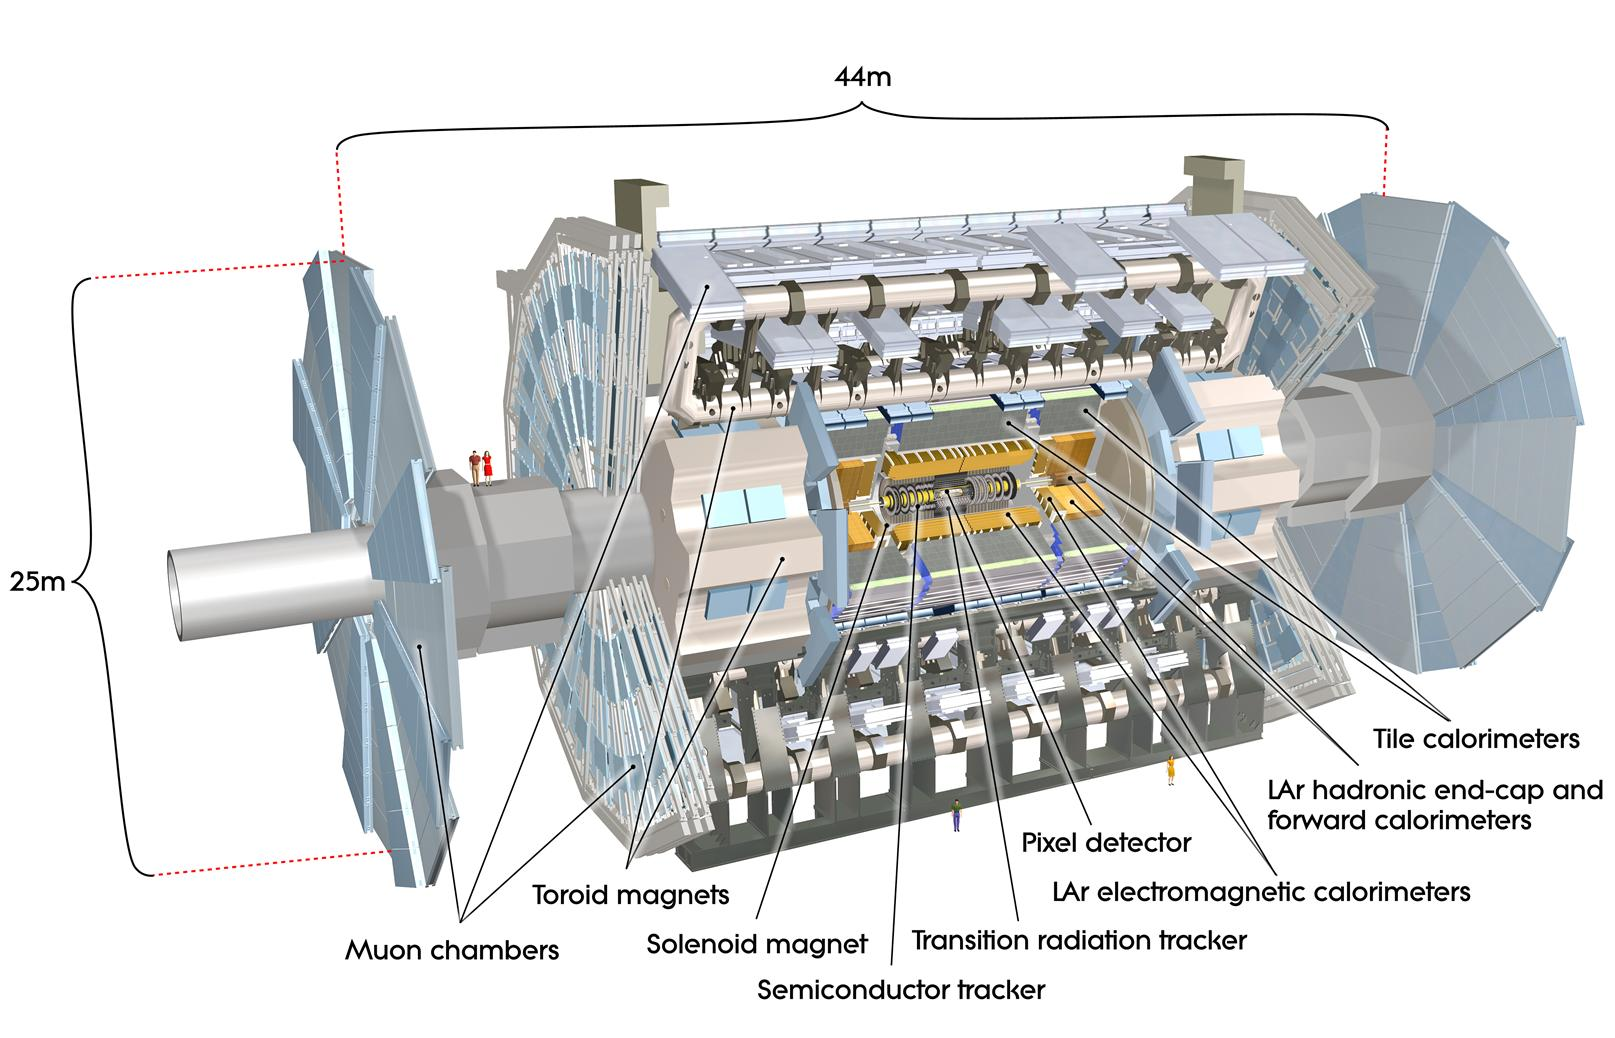
\includegraphics[width=1\linewidth]{images/atlas-detector.jpg}
    \caption{A visual representation of the ATLAS detector at CERN. Reference \cite{CERN_official}.}
    \label{fig:atlasdet}
\end{figure}

The ATLAS detector, shown in figure \ref{fig:atlasdet}, is one of the two general-purpose detectors at the LHC. Inside of it, six different detecting subsystems arranged in layers around the collision point record the path, momentum, and energy of the particles, allowing them to be individually identified and then try to reconstruct what was created back at the collision point.

\subsection{The ATLAS trigger system}\label{ch:trigger}
The interactions in the ATLAS detector create an enormous flow of data. To digest the data, ATLAS uses an advanced trigger system to tell the detector which events to record and which to ignore. Complex data-acquisition and computing systems are then used to analyse the collision events recorded.

Via two levels of filtering: an online trigger (as soon as the event has been recorded) and one offline (after the event has been saved), around 1000 events are being selected as interesting and possibly containing new physics out of the 40 million ones produced per second. %Jet algorithms, described in chapter \ref{ch:reconstruction} aid greatly to that.

Those events are the ones used as input data to the software that will be analysed in this report.
\section{Motivation}
This dissertation was a result of collaboration with the experimental particle physics group of the University of Edinburgh. The group suggested the project, aided in tailoring it as an HPC dissertation, and provided guidance throughout its duration. Also, a personal reason for the choice of this project is the student's ambition to pursue a PhD in experimental particle physics and the desire to comprehend the underlying physics.     

The luminosity of the LHC, which means the number of collisions that occur in a given amount of time, reaches new milestones with every new upgrade. This is done by increasing the number of particles that collide, or decreasing the diameter of the particle beams. This leads to more and more events to be analysed. There is no good reason creating those events if they cannot be processed properly and in time.

Jets are streams of particles emerging from the collision point and account for a considerable part of the analysis. In figure \ref{fig:jets1} jets are presented as light blue cones. Finding new ways to process jets quickly, namely jet reconstruction, is crucial for the future of experimental particle physics. The current dissertation project follows a performance analysis of two particle jet software packages.

The first one is FastJet, currently the most established one in the field and heavily used by the particle physics community. It is a C++ software package consisting of around 2 million lines of code and implementing many optimised jet reconstruction algorithms. The performance analysis of FastJet aimed to understand the reasons keeping it from running even faster, and also why it hasn't been parallelised yet. 


The second software package that was analysed follows a very different direction. It is a neural network that learns how to take as input data the output of different jet algorithms, and forms an unbiased opinion regarding the jet's substructure. It is written in Python with call to Keras, a high-level neural networks API, on top of Tensorfow, an open source machine learning framework. The performance analysis of this neural network aimed to discover any performance bottlenecks.

The university of Edinburgh experimental particles physics group is actively involved in the development of this software package.

\section{Chapters breakdown}

Chapter two, provides some physics insight to make the scope of the project more clear, while chapter three is an introduction to jet algorithms used by both software packages. 

Chapter four is a discussion regarding FastJet, and chapter five describes the performance analysis process that was followed.

Similarly, chapter six explains briefly what an adversarial neural network is and chapter seven introduces the jet substructure adversarial neural network. Chapter eight recites the performance analysis process for the neural network. 

In chapter nine, a discussion following both performance analyses takes place, and chapter ten is brief presentation of the findings.




\chapter{The Underlying Physics }
\section{Particle Collisions}

When trying to understand what the Universe is made of at a fundamental level, one can take ordinary matter and break it up into ever smaller and smaller pieces. But when that is over, very small constituents of matter will be found inside: everything around us is made of molecules, which are in turn made of atoms. Those can be broken into electrons and the nuclei. Every nucleus is composed of protons and neutrons. The two last are made up from quarks and gluons. 

That is not everything nature has to offer though. There are other more exotic particles out there that are not necessarily found inside ordinary matter. Thankfully, there is a convenient way to make a lot of what is possible for the universe to make: by taking advantage of special relativity. If enough energy is brought together in one location in space and time, a lot of what the universe allows can be created. The more energy there is available, the more massive the particles that can be created. See reference \cite{TheLHCmadesimple} for a more in-depth approach, written in everyday language.

This is exactly what is happening at the Large Hadron Collider. Physicists create collisions with as much energy as possible, by accelerating and colliding particles of ordinary matter. A representatino of a particle event can be seen in figure \ref{fig:jets1}. At the LHC protons are chosen because they exist in abundance and they are also heavy enough to radiate much less than electrons.

Since protons are so tiny, most of the times that they are shot at each other, they miss; but in the occasions they do collide, an avalanche of decays takes place. New particles are created from the existing energy, and then decay almost right away into other particles, again and again, until eventually stable particles are reached. The stable particles are the ones observed by the particle detectors.

\begin{figure}[H]
\centering
  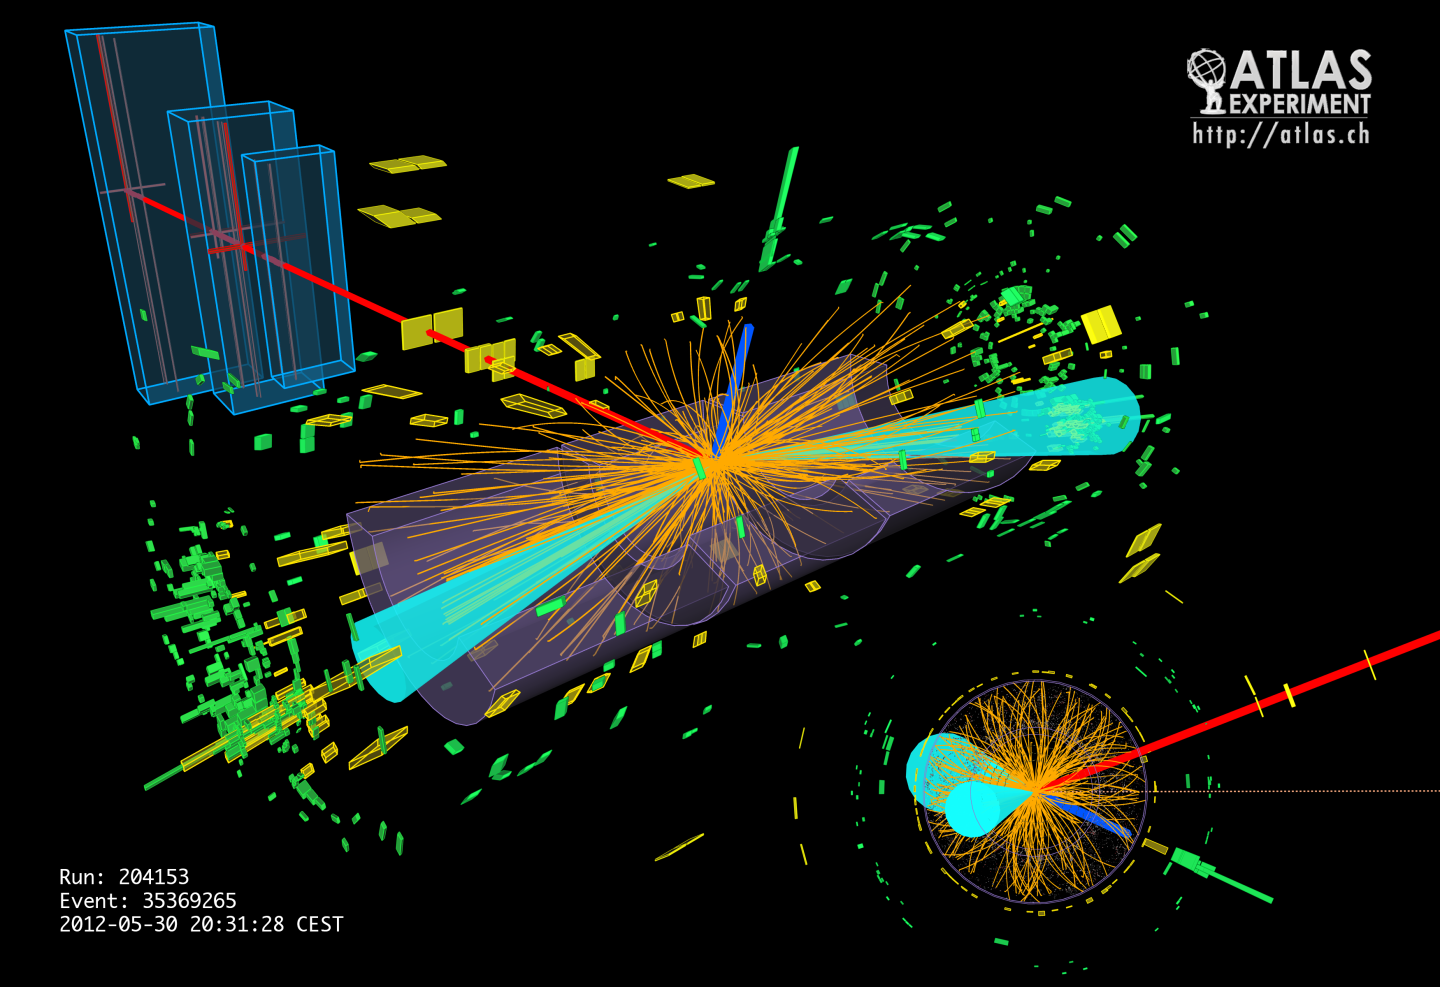
\includegraphics[width=\linewidth]{images/jets1.png}
  \caption{A visual representation of the particles flying out from the collision point. As can be seen, different types of particles are identified using different detecting systems (shown with distinct colours). The light blue cones represent particle jets. Reference \cite{aad2008atlas}.}
   \label{fig:jets1}
\end{figure}


\section{Particle Jets}\label{ch:particlejets}
The particles produced from the collisions fly out from the collision point in different ways depending on their type. Perhaps one of the most impressive and easily distinguishable observed structure is particle jets.  The formal definition of a jet is "a collimated spray of stable particles arising from the fragmentation and hadronisation of a parton (quark or gluon) after a collision" \cite{atkin2015review}. Essentially, a jet is a spray of particles, flying away from the collision point, forming a narrow beam. If the shape of a jet would be visualised it would look like one of the sky blue cones in figure \ref{fig:jets1}. This section aims to provide a basic understanding of that phenomenon.


Protons and neutrons are composite objects built out of three quarks, which are bound together by gluons. Quarks and gluons are assumed to be fundamental particles, meaning that they have no internal substructure. If one tries to pull a quark away from the rest they act like springs; the further and further a quark is pulled away, the greater the force with which it wants to “snap” back to the other quarks. The more the energy that is put to the system to get these particles further apart, the stronger and stronger the attractive force gets \cite{TheLHCmadesimplefreequarks,jetalltheway}.

In the case that someone insists on pulling the quarks further and further apart, this action will eventually require so much energy to be put to the system that, eventually, it will be enough for a new particle-antiparticle pair to be created out of the vacuum with it.%, rather than the quarks being pulled further apart.

This is the mechanism behind jet formation. In the collision points of LHC, every once in a while, there will be a huge jet of particles that fly off from the high-energy collision point. How do so many particles get together in one place? Because for a very brief moment, a high energy quark was created, and it began to pull all these particle-antiparticle pairs out of the vacuum. \cite{TheLHCmadesimplefreequarks,jets}.


\section{Boosted Particles and jet substructure}\label{ch:fatjet}

Physicists use \textbf{boost} to describe Lorentz transformations in relativity, meaning a conversion between two frames of reference that travel with different velocities. A \textbf{boosted particle} refers to a particle that travels at high speed through the laboratory. As the Large Hadron Collider at CERN operates at a very high beam energy, it is very common that the particles produced come out with very large velocity, thus boosted.

Typically, the heavy particles that interest physicists are not observed themselves, but decay into other particles, which in turn are captured by the particle detectors. The boost of the mother particle changes the way its decay products are observed in an experiment. 

To make this clearer, a heavy particle can be imagined decaying to two lighter blue particles, as in figure \ref{fig:boost}. If the heavy particle is at rest relative to the laboratory (figure \ref{fig:boost} left), because of conservation of momentum, the two decay products shoot off in opposite directions. If one is observed in the upper half of the detector, the other will be spotted in the lower half. On the other hand, if the heavy particle is boosted (figure \ref{fig:boost} right), the topology of the decay is quite different. Given a large enough boost, both daughter particles are emitted in the same direction. 

%To make this clearer, a heavy pink (with the solid circle) particle can be imagined decaying to two lighter blue (with the open circle) particles, as in figure \ref{fig:boost}. If the pink particle is at rest relative to the laboratory (figure \ref{fig:boost} left), because of conservation of momentum, the two decay products shoot off in opposite directions. If one is observed in the upper half of the detector, the other will be spotted in the lower half. On the other hand, if the pink particle is boosted (figure \ref{fig:boost} right), the topology of the decay is quite different. Both daughter particles are emitted in the same direction. 


For sufficiently large boost, both daughter particles will be very close together in the detector. If a boosted particle decays into quarks and anti-quarks their jets will overlap, up to the point where one can no longer distinguish the individual jets. As a result, the whole decay fuses into a single jet with substructure, meaning that it consists of more than one or more subjets. These jets are called  "fat" jets \cite{boosted}.

\begin{figure}[H]
  \centering
  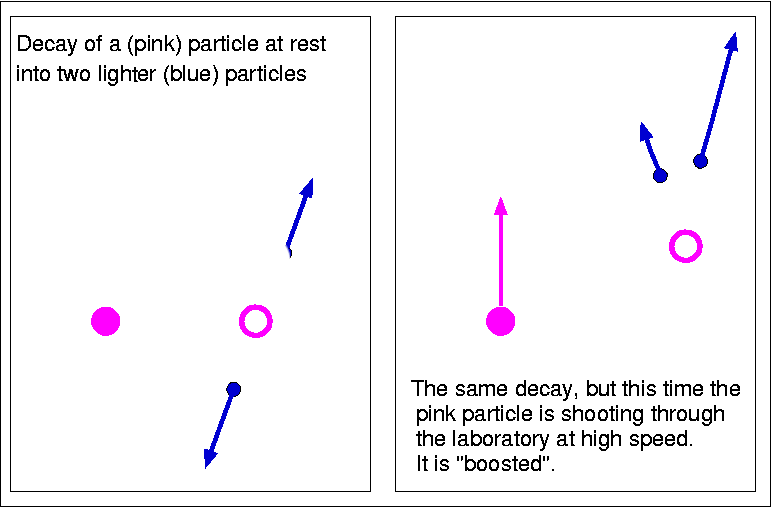
\includegraphics[width=\textwidth]{images/boost.png}
  \caption{A heavy pink (with the solid circle) particle decays to two lighter blue (with the open circle) particles. If the heavy pink particle is at rest relative to the laboratory (figure \ref{fig:boost} left), because of conservation of momentum, the two decay products shoot off in opposite directions. If one is observed in the upper half of the detector, the other will be spotted in the lower half. On the other hand, if the heavy pink particle is boosted (figure \ref{fig:boost} right), the topology of the decay is quite different. Both daughter particles are emitted in the same direction. Reference \cite{boosted}.}
  \label{fig:boost}
\end{figure}

The experiments only detect jets, but physicists are interested in the events that produced them. As a result, it is essential to be able to identify jets and reconstruct what produced them. This requires software packages such as FastJet. Algorithms, as well as being accurate, they need to operate rapidly to cope with the number of events. In the next chapter the algorithms implemented by FastJet are discussed.


\begin{comment}

\section{Boosted Higgs Analysis} \label{ch:higgs_analysis}
The Higgs boson's existence was confirmed back in 2012 by both the ATLAS and CMS experiments. (Un)surprisingly, the Higgs analysis did not stop there. There is currently a huge ongoing research studying a variety of its decays, hunting possible heavier charged Higgs bossons and much more.

Since the Higgs boson requires an enormous amount of energy to be produced, it often happens that it is created with a lot of Kinetic energy or, alternatively said, boosted.

\end{comment}